\documentclass[11pt]{article}
\usepackage{eacl2012}
\usepackage{times}
\usepackage{latexsym}
\usepackage{amsmath}
\usepackage{tikz}
\usepackage{graphicx}
\usepackage{multirow}
\usepackage{url}
\DeclareMathOperator*{\argmax}{arg\,max}
\setlength\titlebox{6.5cm}    % Expanding the titlebox

\title{Visualising Typological Relationships: Plotting WALS with Heat Maps}

% \author{Richard Littauer \\
% University of Saarland\\
% Computational Linguistics Department\\
% Saarbr\"ucken, Germany\\
%   {\tt richard.littauer@gmail.com} \\\And
% Rory Turnbull \\
% Ohio State University\\
% Department of Linguistics\\
% Columbus, Ohio\\
%   {\tt turnbull@ling.osu.edu} \\\AND
% Alexis Palmer\\
% University of Saarland\\
% Computational Linguistics Department\\
% Saarbr\"ucken, Germany\\
%   {\tt apalmer@coli.uni-sb.de}\\} 

\date{}

\begin{document}
\maketitle

\begin{abstract}
This paper presents a novel way of visualising relationships between languages. The key innovation of the visualisation is that it brings geographic, phylogenetic, and linguistic data together into a single image, allowing a new visual perspective on linguistic typology. The data presented here is extracted from the World Atlas of Language Structures (WALS)~\cite{wals-2011}. After pruning due to low coverage of WALS, we filter data about linguistic structures and attributes by geographical proximity in order to get at areal typological effects. The data are displayed in heat maps which reflect the strength of similarity between languages for different linguistic aspects. Finally, these are annotated for language family membership. The images so produced allow a new perspective on the data which we hope may facilitate interesting findings and perhaps even illuminate new areas of research.
\end{abstract}

\section{Introduction}

This paper presents a novel way of visualising relationships between languages. Relationships between languages can be understood with respect to linguistic features of the languages, their geographical proximity, and their status with respect to historical development. The visualisations presented in this paper are the first to bring together these three perspectives into a single image. One line of recent work brings computational methods to bear on the formation and use of large typological databases, often using sophisticated statistical techniques to discover relations between languages \cite[among others]{cysouw2011,daume07implication,daume09areal}, and another line of work uses typological data in natural language processing \cite[for example]{georgi:etal:10,lewis:xia:08}, but we are unaware of any previous approaches to visually presenting the resulting data. Here, we address this gap by using data from the World Atlas of Language Structures \cite{wals-2011} to develop heat maps that can visually show the interconnected relationships between languages and language families. 

The main envisioned application of our visualisations is in the area of linguistic typology. Typology has been used to derive implications about possible languages, and about the ordering of the human mind. Different theorists have taken different views on the relationship between typology and the universality of languages. For example, Greenberg \shortcite{greenberg}, a foundational work in the field, identifies a number of cross-linguistic typological properties and implications and aims to present them as truly universal -- relevant for \textit{all} languages. In a similar vein, typological universals have been employed as evidence in a generative story regarding language learning \cite{chomsky}.

Taking a different perspective, Dunn {\it et al} \shortcite{Dunn_Greenhill_Levinson_Gray_2011} argued that a language's typology relies upon the previous generations' language more than on any biological, environmental or cognitive constraints, and that there are pathways which are generally followed in language change based on the previous parent language. What these arguments have in common is a reliance on a view of linguistic typology that is potentially restricted in its scope, due to insufficient access to broad-scale empirical data, covering many features of many languages of the world. 

The most comprehensive computational resource for linguistic typology currently available is the World Atlas of Language Structures (WALS).\footnote{As of 2008, WALS is browsable online (\url{http://www.wals.info}).}  WALS is a large database of details of structural properties of several thousand languages \cite{wals-2011}. The properties were collected from descriptive sources by the project's 55 authors. However, for the several thousand languages in WALS, there is only about 16\% of the possible features filled---the data are \emph{sparse}, and the sparsity of the data of course makes it difficult to perform reliable statistical analysis. One way to work around this limitation is to seek meaningful visualisations of the data in WALS, instead of simply relying on raw numbers. This is our approach. 

In this paper, we first discuss in more detail the source data and the types of information to be extracted, followed by a discussion of some difficulties presented by the available data and our approaches for addressing those difficulties. Finally, we show the resulting visualisations.

\section{Aspects of the Visualisations}

The visualisations described here bring together three types of information: linguistic features, geographical distance, and phylogenetic distance. For the current study, all three types of information are extracted from the WALS database. In future work, we may explore the use of alternate sources such as Ethnologue \cite{ethnologue} or MultiTree \shortcite{multitree} for alternate phylogenetic hierarchies. 

% The above sentence is vague. 16% of what? What does it mean for the features to be filled? Only 16% of the features are "full"? Only 16% of languages have full descriptions for each feature?

% Dealing with sparse data is a computational problem, as any statistical information drawn from the database will, to a large extent, be an artefact of the database. For instance, if half of the languages were marked as having uvular stops (unlikely), and then in reality if all other languages not in the database had uvular stops, then the knowledge we would glean from the database would be significantly false and misleading. Given that there are around 6,000 languages in the world, the amount of languages on WALS means that this is a serious concern. Many researchers in recent years have been developing work-arounds for sparse databases; often because languages with low resources have a similar problem. %Cite cite cite

% The above para is also unclear. The sparsity of data problem just sounds like a sampling problem, which is endemic to all of science. Also, can we state at some point *how many* lgs are in WALS? that's not clear.

%\item visualisation
%\item what visualisation can do for us
%\item Heat Maps  where they come from, what they are doing here

%192 features in WALS
% At the time of submission, there were 81,828 datapoints for 2,678 languages (an average of 28 per language). At least one feature, the most populated, had data for 1,519 languages. There were 144 different chapters, each containing values for different, related features. It can be seen easily from these numbers that the data on WALS is \emph{sparse}. Ignoring the fact that a language having certain features will cancel out the possibility or probability of others, that means that the WALS possible data is only 15.8\% represented in the database.

\subsection{Linguistic features}
At the time of submission, WALS contained information for 2678 languages. The linguistic features covered in WALS range from phonetic and phonological features, over some lexical and morphological features, to syntactic structures, word order tendencies, and other structural questions. A total of 192 features are represented, grouped in 144 different chapters, with each chapter addressing a set of related features. 

The coverage of features/chapters varies dramatically across the languages, with an average of 28 feature values per language. The most populated feature has data for 1519 languages. Because of the extreme sparsity of the data, we restricted our treatment to only languages with values for 30\% or more of the available features. 


\subsection{Geographic distance}
Geographic distance is an important aspect of typological study because neighbouring  languages often come to share linguistic features, even in the absence of genetic relationship between the languages. Each language in WALS is associated with a geographical coordinate representing a central point for the main population of speakers of that language. We use these figures for determining geographic distance between two languages. A crucial aspect of our visualisations is that we produce them only for sets of languages within a reasonable geographic proximity (and with sufficient featural coverage within WALS).

For this study, we try two approaches to clustering languages according to geographic distance. First, we choose an arbitrary radius in order to create a decision boundary for clustering neighbouring languages. For each language, we fix that language's location as the centroid of the cluster and look at all other languages within the given radius. We found that a radius of 500 kilometers proves to provide a sufficient number of examples even after cleaning low-coverage languages from the WALS data. 

The second approach selects an arbitrary lower bound for the languages in the general area. If a sufficient percentage of the total number of languages in the area remained after cleaning the WALS data, we took this as a useful area and did mapping for that area. 
% that would would create a decision boundary to cluster $n$-nearest neighbours. For our purposes, we went with 500km, as this proved to %provide sufficient examples to draw from from cleaned WALS data. We also measured distance by selecting an arbitrary lower threshold for %languages in the general area, and printed the results if the amount of cleaned languages in the area was a certain percentage over the amount of languages in the area total as specified by WALS. 
This number is clearly under-representative of the amount of contact languages, as only half of the world's languages are present in WALS. This proxy was not as good at choosing specific, useful examples, as the $n$-nearest nieghbours, as the languages chosen were often too far away. 
%Haversine Formula - distance on a sphere (earth) http://en.wikipedia.org/wiki/Haversine_formula
% (Vincenty formula would be more accurate (as earth is not a 
% perfect sphere), but much more computationally intense for
% 2678*2678 comparisons.
%   http://www.codecodex.com/wiki/Calculate_Distance_Between_Two_Points_on_a_Globe#Python
%Note - reprint the data with this formula worked in, as it makes more sense than what you're doing at the moment.

\subsection{Phylogenetic distance}

Languages are related phylogenetically either vertically, by lineage, or horizontally, by contact. In WALS, each language is placed in a tree hierarchy that specifies phylogenetic relations. In the WALS data files, this is specified by linking at three different levels: family, such as `Sino-Tibetan', sub-family, such as `Tibeto-Burman', and genus, such as `Northern Naga' . % Provisional tree hierarchies were also drawn from Ethnologue \cite{ethnologue} and MultiTree \cite{multitree}, but due to the low amount of overlap between non-sparse WALS entries and the possible alternative hierarchies drawn from Ethnologue or MultiTree, only the phylogenetic relations from WALS were used.
% If we didn't use the ethnologue or multitree data, we don't need to mention it.
% Well, we did run it - I don't know, I feel like it's important to mention that it is a neg result for new results mapping to Ethnologue. I wish I had known this before, by reading it in some other article. 

%Information about Ethnologue scrape %provided by steven moran -need to get the details
The WALS phylogenetic hierarchies do not take into account language contact. For that, we used geographic coordinates, which are present on WALS, as a proxy for contact. 
%\item Longitude and latitude, and how it is measured
%Distance:
%    For each language, the distance has been calculated. Currently we have a
%    2678x2678 matrix, which is a little large.



\section{Producing the heat maps}

Because of the sparse coverage of the WALS data, we focus our visualisations on languages with a reasonable number of filled features.
Ignoring the fact that a language having certain features will cancel out the possibility or probability of others, that means that the WALS possible data is only 15.8\% represented in the database. %The data was represented as a range of numbers indicating the type of each feature.
 The methodology discussed in this section is relevant only for languages with values for at least 30\% of all possible feature categories. 
All data was downloaded freely from WALS, all coding was done in either Python or R. The code was not computationally expensive to run, and the programming languages and methods are quite accessible. All code is available in a public repository, links to which will be released once anonymisation is no longer required.

\subsection{Geographically-organized heat maps}
For the geographic distance maps, for each language present in the cleaned data, we selected all possible languages that lay within 500km, and sorted these languages until only the 15 closest neighbors were selected. For phylogenetic distances, for each language we searched for other languages coming from the same family, subfamily, or genus. In either case, the subset that fit these requirements was a mere handful. We have chosen to graph these examples, as they most fully show the use of our visualisations. We picked features to graph from among the resulting languages based on how common they were across the selected languages. 

%\item Description of typological data %Insert example? here. Probably. 

Each final list was then resorted. In the geographic case, the source language was centered in the map. This was due to one of the primary issues with using distance on a two dimensional graph. On the one hand, we would want close languages to be close together on the heat map. However, given the source language Egyptian Arabic, this would mean that Zulu, Saami, Mohawk, and Japanese might all roughly be placed next to each other on the map. This also means that Japanese might be placed next to Mohawk, and Mohawk again next to Korean. This is not ideal, and was the main justification for limiting the sphere of possible geographical languages to a reasonable distance, given the data. Language families were put as a bar at the top of the image, in order to show relations that might otherwise not be obvious.


\subsection{Phylogenetically-organized heat maps}

The phylogenetic example was sorted by geographical position, as well. In this case, we first plotted the subset of languages on a world map, and examined which groups had the most linear structure. We then arranged that group according to cardinal directions; here, we mapped from North to South. This is a better proxy in this case than centering the data, as it more clearly shows languages that would be in contact with each other. 


%\item Information about WALS data
\subsection{Sparse data}

%192 features in WALS

\begin{figure}[h]
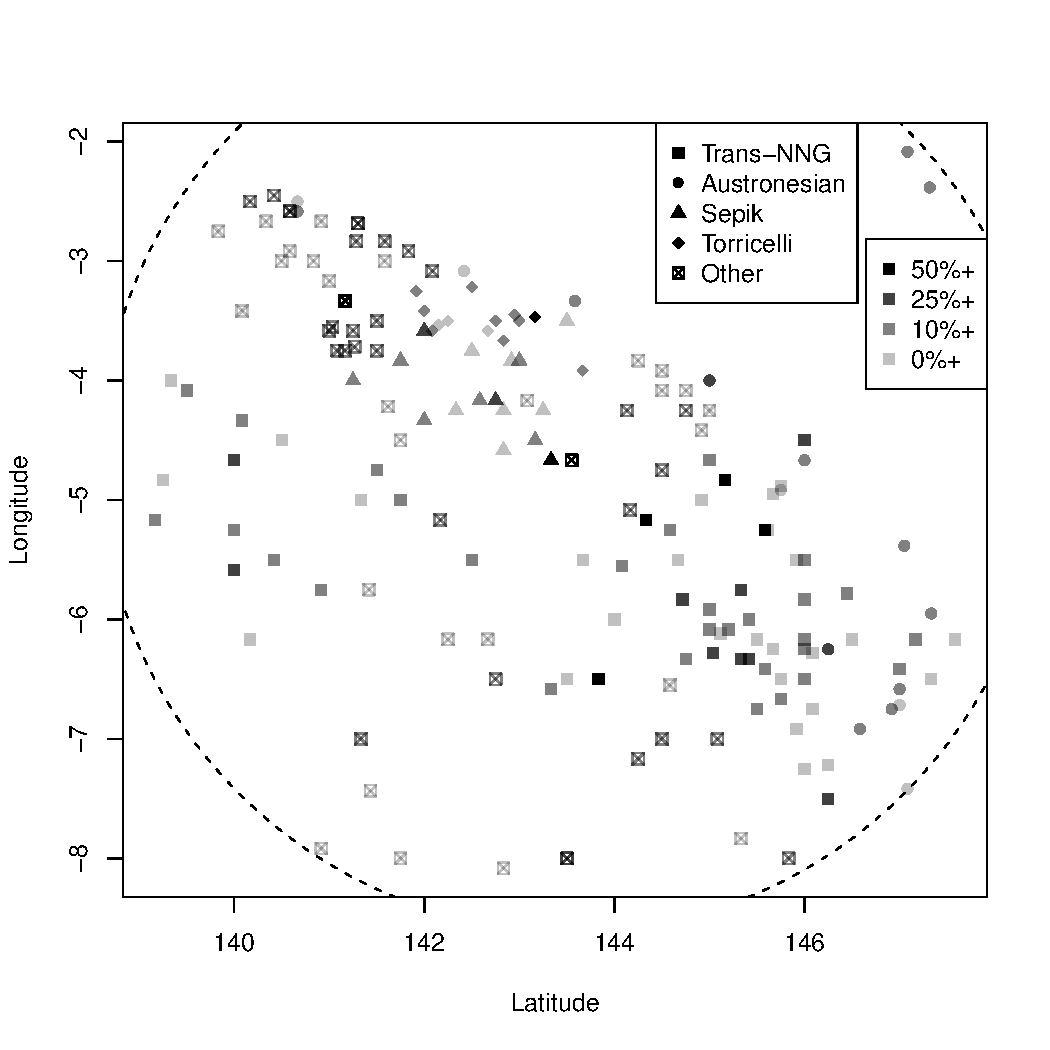
\includegraphics[width=3.1in]
{graph1sparse.pdf} 
\caption{Sparse Data} 
\label{fig:sparse} 
\end{figure}

In Fig. \ref{fig:sparse}, we have plotted out the neighbouring languages for the most populous language area represented on WALS by longitude and latitude. The center language, Yimas, is a Trans New Guinean language, and is the center for the graph. The odd clustering is due to the Pacific Ocean - such geographical features limit the usefulness of distance as a measure. Another limit is the range of each language, which is not represented here, as each language is given only a single geographical coordinate that does not indicate the area over which the language resides, nor how many other languages coexist with it.

For each language within 500km, represented here by the dotted circle, the amount of features filled in WALS is shown. The majority have less than 50\% filled - there are only 171 such languages in WALS. This graph does not include languages not in WALS. It ought to be clear from this that the data in WALS is too sparse to draw immediate conclusions from, which furthers the need for visualizations. 

Drawing a heat map where only 16\%~ of the features are available would be of little use. There are two options for dealing with this: to collapse the feature values in some way, or to select for languages that have a higher percentage of data filled than the average language. We opted for the second choice, and \emph{cleaned}  the file until it contained only languages that had at least 30\% as a lower bound of all of their entries filled. This cleaned data was then used in the other functions.  

\section{Results} %Or visualisations?



\begin{figure}[h]
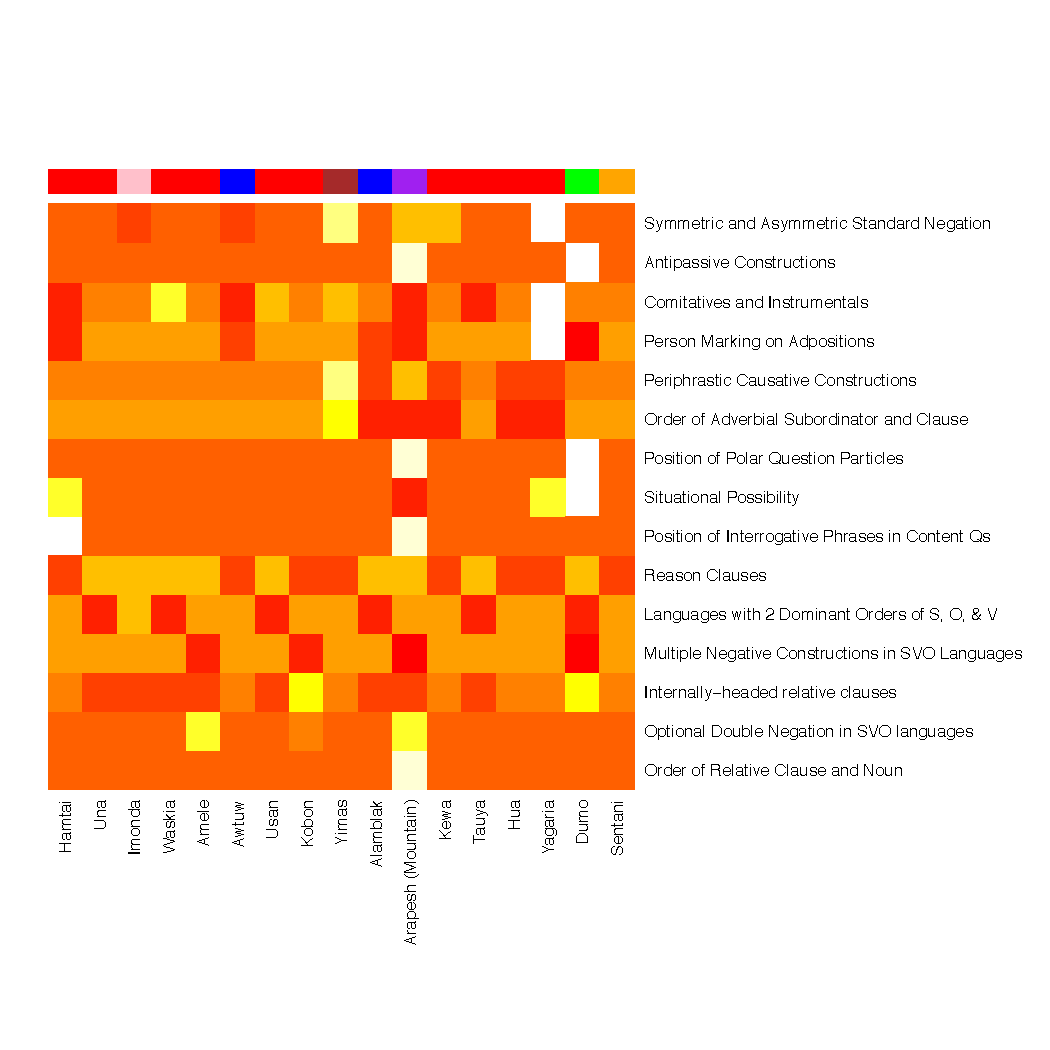
\includegraphics[width=3.1in]
{graph2yimassmall.pdf} 
\caption{Example 1} 
\label{fig:sparse} 
\end{figure}

\begin{figure}[ht!]
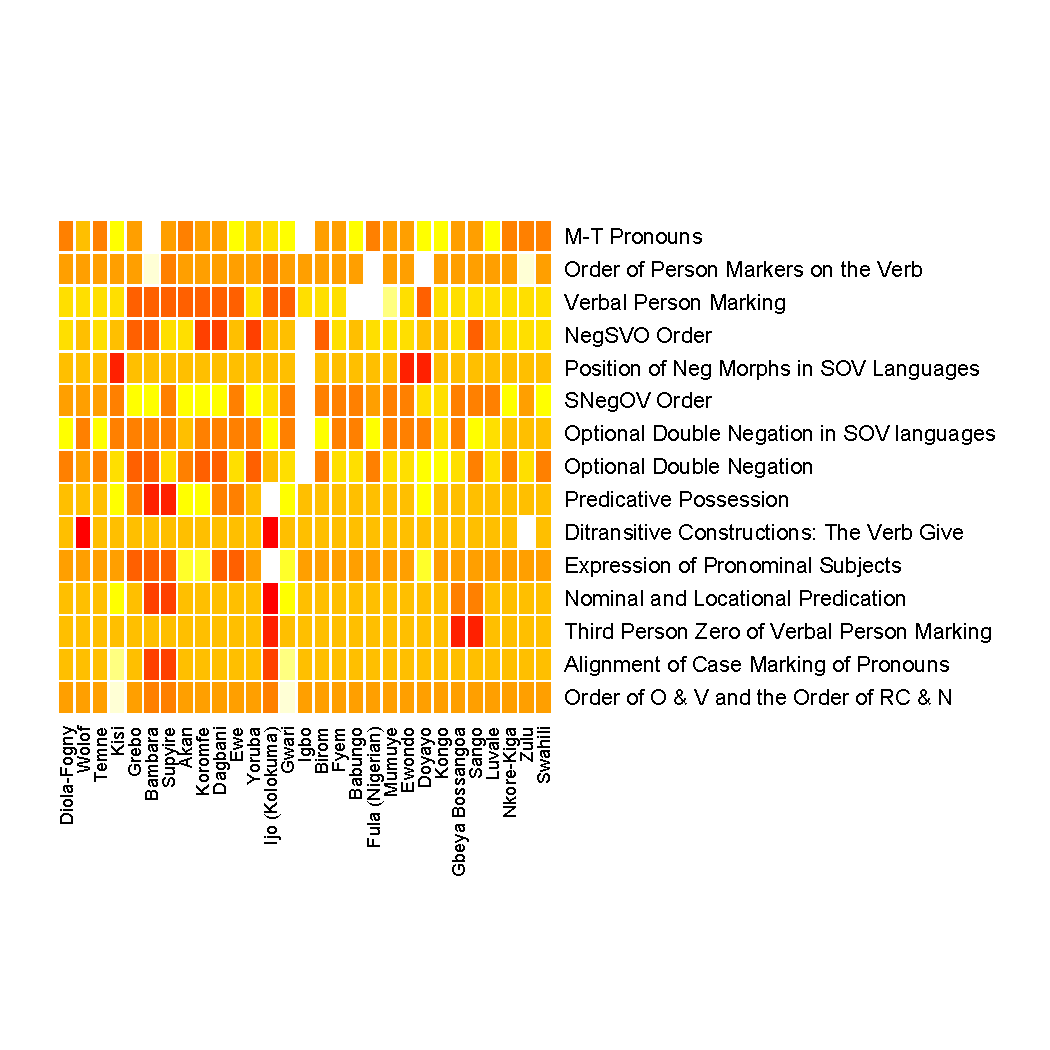
\includegraphics[width=3.1in]
{graph3nigercongosmall.pdf} 
\caption{Example 1} 
\label{fig:sparse} 
\end{figure}


\section{Conclusion}
In this paper we present a new method for visualising relationships between languages, representing 

%\begin{itemize}
%\item What these tell us (map by map)
%\item What these tell us, overall - implications
%\item Warnings: sparse data, data not there, etc. 
%\item Future work 
%    We could also plot on a world map, but that would not be a heat map. An
%    option for this would be to color gradiantly based on certain featurs - for
%    instance, color could indicate phoneme size. 
%
%    Another option would be a matrix map of some sort - Again, not a heat map,
%    and beyond the scale of this current study.


\bibliographystyle{acl}
\bibliography{lingviz}

\end{document}
